% Cuckoo filter insert + kick chain (Fan et al. 2014).
\documentclass[border=10pt,tikz]{standalone}
\usepackage{tikz}
\usetikzlibrary{arrows.meta,positioning,fit,backgrounds,calc}

\definecolor{sand}{HTML}{E9DCC4}
\definecolor{sanddeep}{HTML}{D8C7A6}
\definecolor{ebony}{HTML}{121212}
\definecolor{ink}{HTML}{1B1712}
\definecolor{cobalt}{HTML}{003FB8}
\definecolor{amber}{HTML}{6B4500}
\definecolor{teal}{HTML}{00564C}
\definecolor{paper}{HTML}{FBF7EF}

\begin{document}
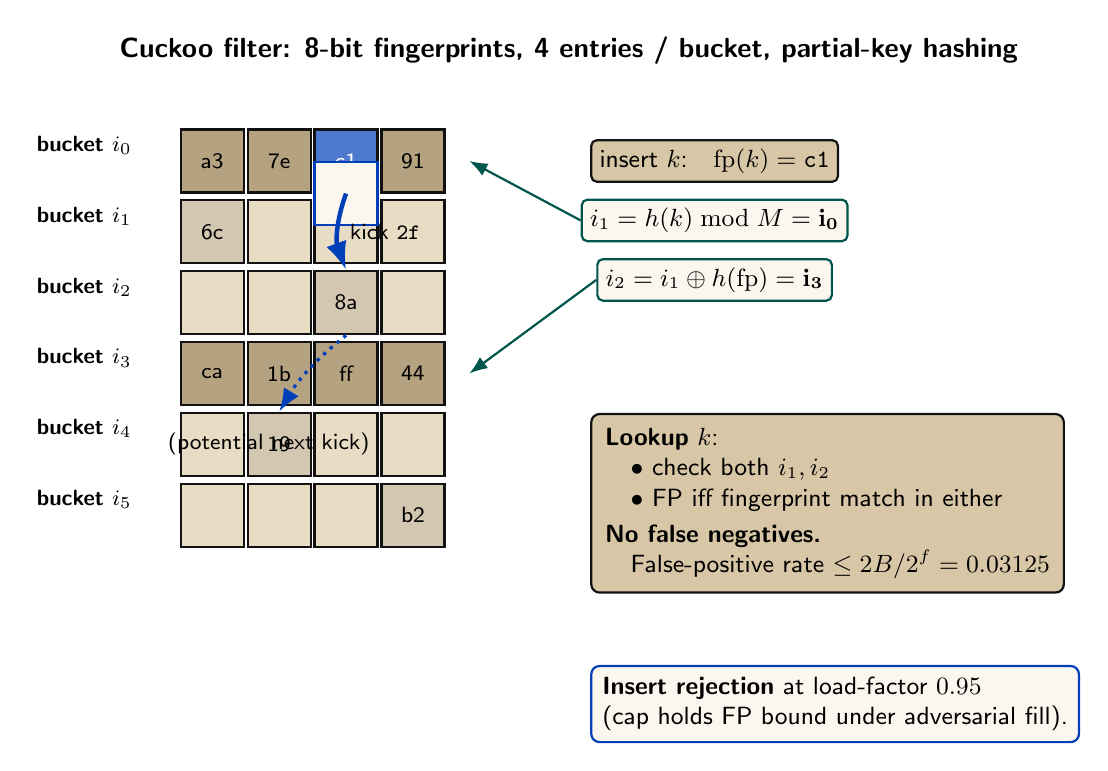
\begin{tikzpicture}[
  font=\sffamily\small,
  slot/.style={draw=ebony,thick,minimum width=8mm,minimum height=8mm,
               fill=paper,inner sep=0pt,font=\sffamily\footnotesize},
  empty/.style={draw=ebony,thick,minimum width=8mm,minimum height=8mm,
                fill=sand,inner sep=0pt},
  bucketlbl/.style={font=\sffamily\footnotesize\bfseries,anchor=east},
  flow/.style={->,>=Latex,thick,draw=cobalt},
  hashflow/.style={->,>=Latex,thick,draw=teal},
]

\node[font=\sffamily\bfseries,anchor=west] at (-0.6,5.0)
  {Cuckoo filter: 8-bit fingerprints, 4 entries / bucket, partial-key hashing};

% Six buckets shown.
\foreach \i/\y in {0/3.6, 1/2.7, 2/1.8, 3/0.9, 4/0.0, 5/-0.9} {
  \node[bucketlbl] at (-0.2,\y+0.2) {bucket~$i_\i$};
  \foreach \s/\xoff in {0/0, 1/0.85, 2/1.7, 3/2.55} {
    \node[empty] (b\i s\s) at (\xoff+0.7, \y) {};
  }
}

% Pre-populate some buckets with fingerprints.
\node[slot,fill=amber!50] at (b0s0)  {a3};
\node[slot,fill=amber!50] at (b0s1)  {7e};
\node[slot,fill=amber!50] at (b0s2)  {2f};
\node[slot,fill=amber!50] at (b0s3)  {91};

\node[slot,fill=amber!50] at (b3s0)  {ca};
\node[slot,fill=amber!50] at (b3s1)  {1b};
\node[slot,fill=amber!50] at (b3s2)  {ff};
\node[slot,fill=amber!50] at (b3s3)  {44};

\node[slot,fill=amber!30] at (b1s0)  {6c};
\node[slot,fill=amber!30] at (b2s2)  {8a};
\node[slot,fill=amber!30] at (b4s1)  {19};
\node[slot,fill=amber!30] at (b5s3)  {b2};

% Insert key — new fingerprint highlighted.
\node[draw=ebony,thick,fill=sanddeep,rounded corners=2pt,
      minimum width=22mm,inner sep=3pt,
      anchor=west] (key) at (5.5,3.6)
  {insert $k$:\\[1pt]\quad $\mathrm{fp}(k)=\mathtt{c1}$};

\node[draw=teal,thick,fill=paper,rounded corners=2pt,inner sep=3pt,
      anchor=west,below=2mm of key] (h1)
  {$i_1 = h(k) \bmod M = \mathbf{i_0}$};
\node[draw=teal,thick,fill=paper,rounded corners=2pt,inner sep=3pt,
      anchor=west,below=2mm of h1] (h2)
  {$i_2 = i_1 \oplus h(\mathrm{fp}) = \mathbf{i_3}$};

% Both candidate buckets are FULL (b0 and b3 are full).
\draw[hashflow] (h1.west) -- ($(b0s3.east)+(0.3,0)$);
\draw[hashflow] (h2.west) -- ($(b3s3.east)+(0.3,0)$);

% Kick chain: evict from b0 -> goes to its alternate.
\node[slot,fill=cobalt!70,text=white] at (b0s2) {c1};   % new fp lands here
\node[slot,draw=cobalt,thick,fill=paper] (kicked) at (b0s2.south) {};

% Evicted "2f" arrow to bucket 2 (its alternate).
\draw[flow,line width=1.6pt] (b0s2.south) to[bend right=20]
  node[right,font=\sffamily\footnotesize]
  {kick \texttt{2f}} (b2s2.north);

% Then bucket 2 had "8a" — would chain if needed, dotted to show.
\draw[flow,line width=1.2pt,dotted] (b2s2.south)
  to[bend right=10] (b4s1.north)
  node[right,pos=0.5,font=\sffamily\footnotesize]
    {(potential next kick)};

% Lookup property
\node[draw=ebony,thick,fill=sanddeep,rounded corners=3pt,inner sep=5pt,
      align=left,anchor=north west,minimum width=58mm]
  at (5.5,0.4)
  {{\bfseries Lookup} $k$:
   \\\quad$\bullet$ check both $i_1, i_2$
   \\\quad$\bullet$ FP iff fingerprint match in either
   \\[2pt]{\bfseries No false negatives.}\\
   \quad False-positive rate $\leq 2B / 2^f = 0.03125$};

% Header right side: rejection ceiling
\node[draw=cobalt,thick,fill=paper,rounded corners=3pt,inner sep=4pt,
      align=left,anchor=north west]
  at (5.5,-2.8)
  {{\bfseries Insert rejection} at load-factor $0.95$\\
   (cap holds FP bound under adversarial fill).};

\end{tikzpicture}
\end{document}
